\documentclass[10pt,twocolumn,letterpaper]{article}

\usepackage{cvpr}
\usepackage{times}
\usepackage{epsfig}
\usepackage{graphicx}
\usepackage{amsmath}
\usepackage{amssymb}
\usepackage{listings}

% Include other packages here, before hyperref.

% If you comment hyperref and then uncomment it, you should delete
% egpaper.aux before re-running latex.  (Or just hit 'q' on the first latex
% run, let it finish, and you should be clear).
\usepackage[breaklinks=true,bookmarks=false,hidelinks]{hyperref}

\cvprfinalcopy % *** Uncomment this line for the final submission

\def\cvprPaperID{****} % *** Enter the CVPR Paper ID here
\def\httilde{\mbox{\tt\raisebox{-.5ex}{\symbol{126}}}}

% Pages are numbered in submission mode, and unnumbered in camera-ready
%\ifcvprfinal\pagestyle{empty}\fi
\setcounter{page}{1}
\begin{document}

%%%%%%%%% TITLE
\title{ Semantic Segmentation for Unnamed Surface Vessle Navigation}

\author{Martin Cote\\
ME780 Perception For Autonomous Driving\\
University of Waterloo\\
{\tt\small m4cote@uwaterloo.ca}
}

\maketitle
%\thispagestyle{empty}

%%%%%%%%% INTRODUCTION
%This section introduces your problem, and the overall
%plan for approaching your problem.

\section{Introduction}
For my final project in ME780, I plan to address the task of semantic segmentation
for the use of autonomous navigation of an unmanned surface vessel (USV). I will be 
doing pixel wise classifications of images from a camera mounted to the USV. For the
purpose of this project, I will only require 2 classes, water and other. This has 
several useful applications for marine industry, such as remote surveys. Classifications
of open water is a part of the of the full stack required to do safe marine autonomy,
similar to classifying drivable roads in autonomous driving applications. This report
will discuss the proposed strategy to be implemented, as well as the current progress 
to this date.

%-------------------------------------------------------------------------
%%%%%%%%% PROBLEM STATEMENT
%Describe your problem precisely specifying the
%dataset to be used, expected results and evaluation.

\section{Problem Statement }
This project is largely motivated by future projects from my place of employment.
I work for the Clearpath robotics, in the research solutions department. We build 
custom robots for the use in robotics research. However we are now looking
towards the remote survey industry, that is using robotics to remotely survey
environments that are too dirty, dull or dangerous for humans. One such task is 
remote marine surveys, wherein a USV is used to collect data from a body of water
while the operator can stay safely on shore. Clearly a very important part of this
task is to determine if the USV has clear water ahead of it, or it will risk 
running aground.

I therefore propose to use concepts discussed in ME780, Perception For Autonomous Driving,
and adapt them for use on a marine vehicle in bodies of water. My goal for this project
is to implement a convolution neural network to make pixel wise classification of an image
from on onboard camera as either "water" or "other". To the best of my knowledge, there is no
dataset publicly available to be used for this task, therefore a large portion of my project will be
collecting and preparing data to be used for training, testing and evaluation of my network. 
My network will be evaluated on both run time and accuracy, however as the intent is to do
live on board semantic segmentation, minimizing runtime will be prioritised. I expect this
implementation to be able to do classifications with sufficient level of accuracy, however
minimizing the runtime to be able to do live classifications may be more challenging.


%-------------------------------------------------------------------------
%%%%%%%%% Technical approach
%Describe the methods you intend to apply to
%solve the given problem.

\section{Technical Approach}
\subsection{Data Collection}
As previously mentioned, there is no publicly available dataset for use in a marine
environment to the best of my knowledge, therefore the first part of this project
will be collecting such a dataset! To do so, I'll be using Clearpath Robotics's
Heron platform with an onboard Point Grey Chameleon camera as shown in ~\ref{fig:heron}

\begin{figure}[h]	
\begin{center}
  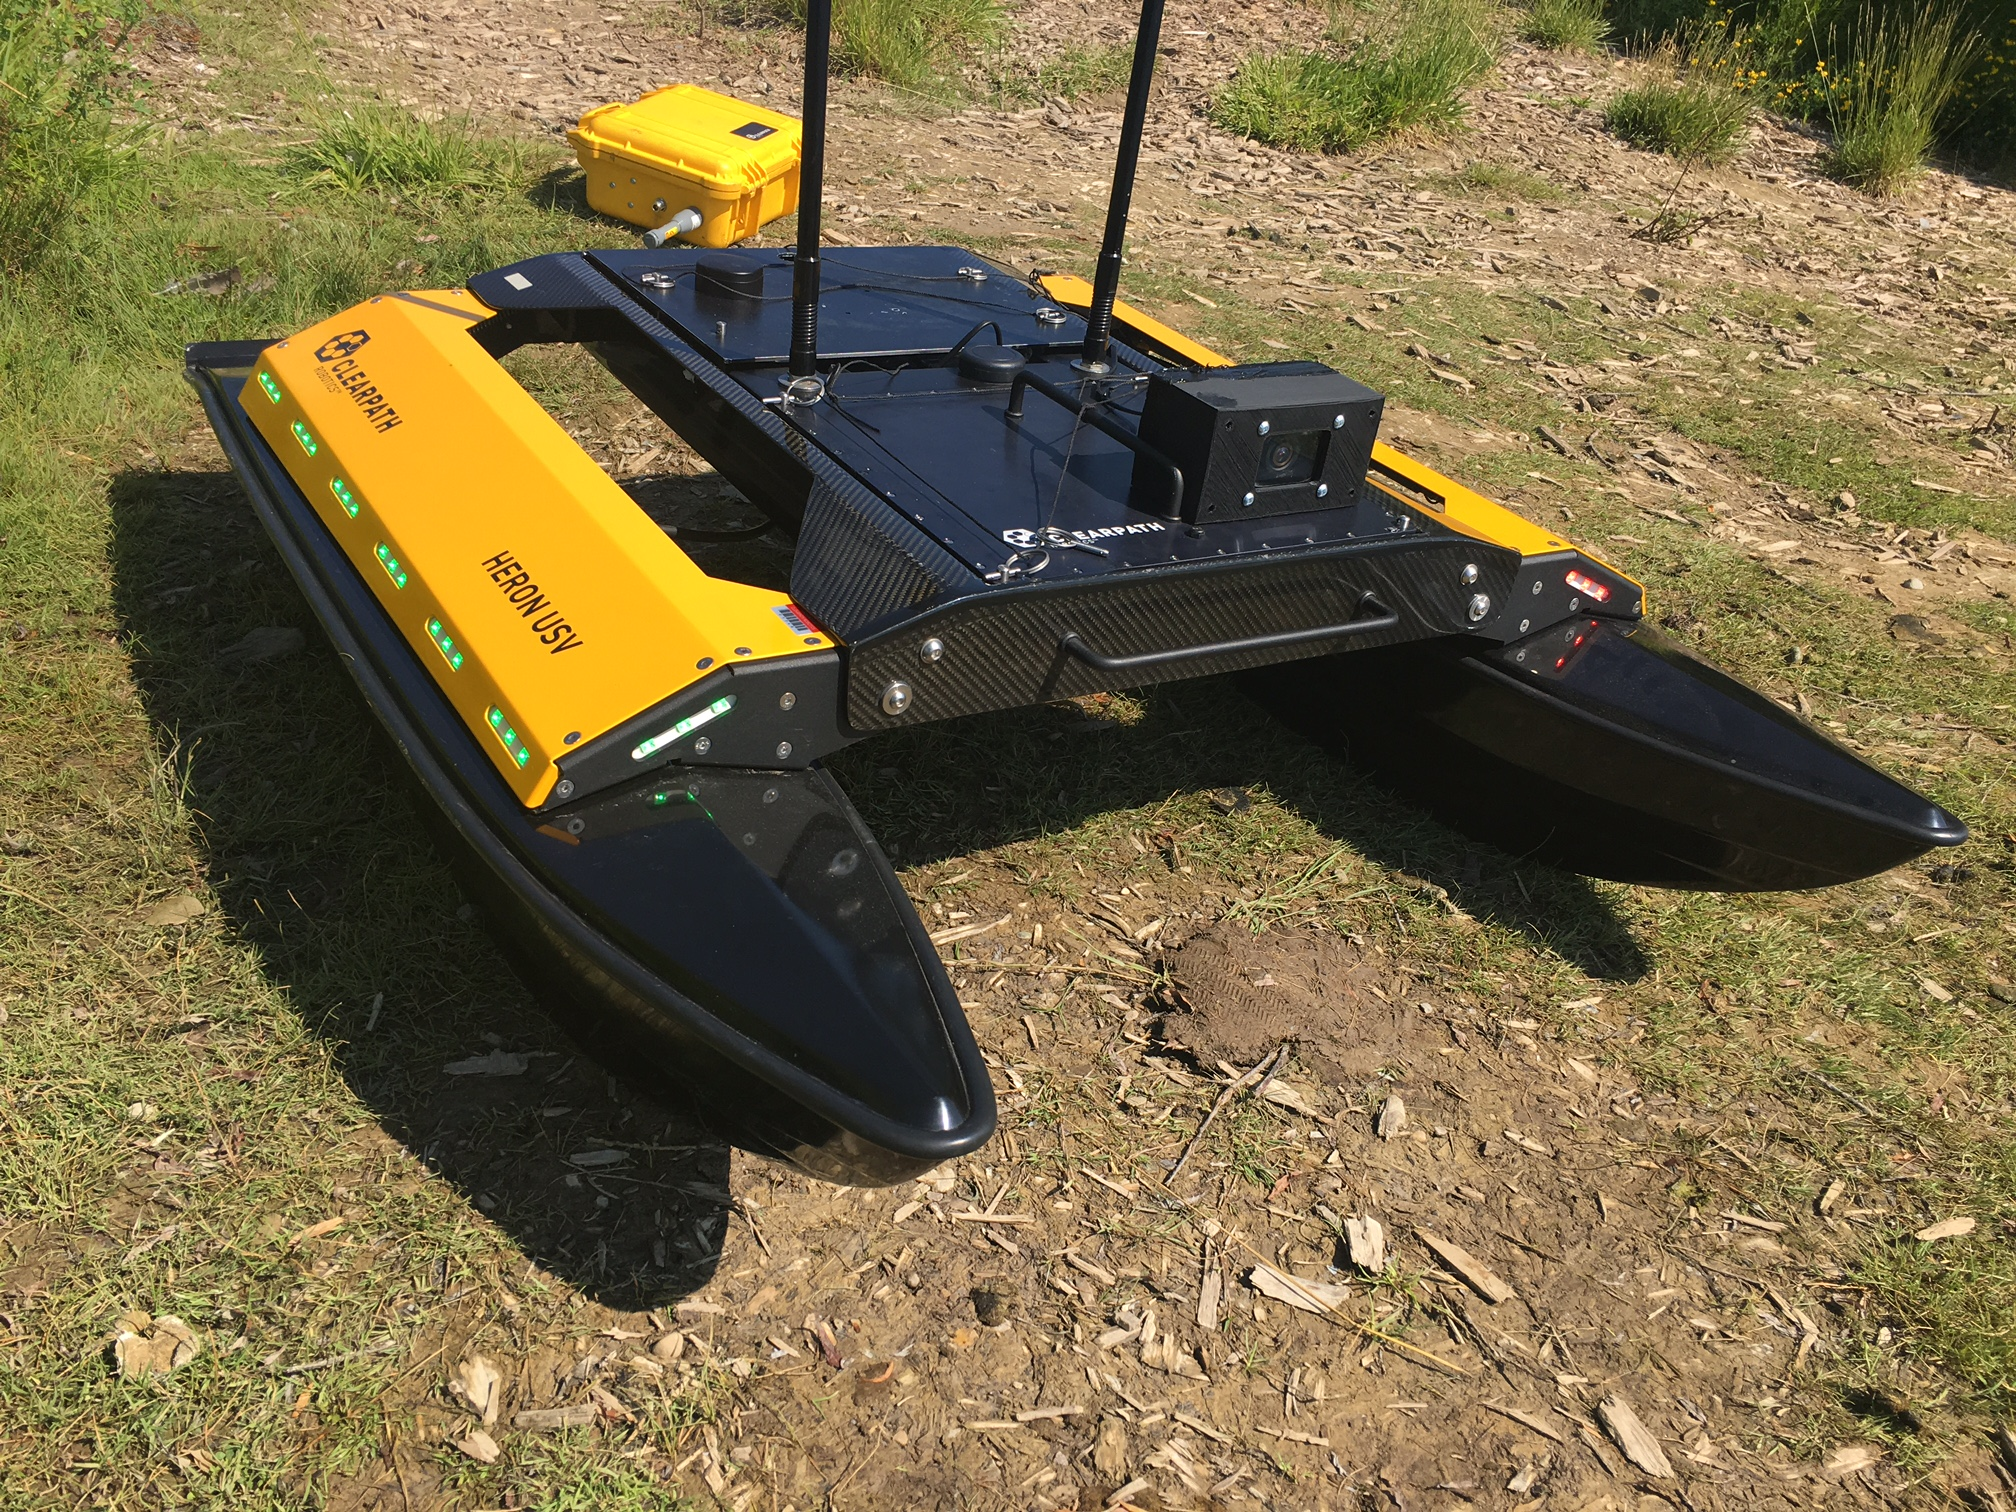
\includegraphics[width=1.0\linewidth]{heron.JPG}
\end{center}
   \caption{Clearpath Robotics's Heron with mounted Camera for marine data collection}
\label{fig:heron}
\end{figure}


The data will be collected in a ROS bag, along with other important ROS topics that may be used
for later stages on the project. The ROS topic \verb|camera\image_color|, will be extracted and 
converted into a mp4 file using the \verb|bag_tools| ROS package ~\cite{bagtools}. PNG images
will then be extracted from the mp4 files at a rate of once every 2 seconds. Repetitive frames
with similar features will be removed.

\subsection{Data Preperations}
Once the images have been collected, they must now be prepared for use with the neural network.
The images must be labelled at a pixel level so 




%-------------------------------------------------------------------------

{\small
\bibliographystyle{ieee}
\bibliography{egbib}
}

\end{document}
